\documentclass[11pt]{article}
\usepackage[textwidth=18.0cm, textheight=23.0cm, top=2.0cm]{geometry}
\usepackage{pst-all}
\usepackage{amssymb}
\usepackage{tikz}
\usepackage{underscore}\begin{document}
\pagestyle{empty}


ClassName: \underline{\textbf{Class_05.2bp-16}}
\par
BinSize: \underline{\textbf{100 × 100}}
\par
ReduceSize: \underline{\textbf{100 × 100}}
\par
TypeNum: \underline{\textbf{40}}
\par
Num: \underline{\textbf{40}}
\par
OutS: \underline{\textbf{100000}}
\par
InS: \underline{\textbf{90638}}
\par
Rate: \underline{\textbf{0.906}}
\par
UB: \underline{\textbf{10}}
\par
LB0: \underline{\textbf{10}}
\par
LB: \underline{\textbf{10}}
\par
LBWithCut: \underline{\textbf{10}}
\par
NodeCut: \underline{\textbf{0}}
\par
ExtendedNodeCnt: \underline{\textbf{1}}
\par
GenNodeCnt: \underline{\textbf{1}}
\par
PrimalNode: \underline{\textbf{0}}
\par
ColumnCount: \underline{\textbf{10}}
\par
TotalCutCount: \underline{\textbf{0}}
\par
RootCutCount: \underline{\textbf{0}}
\par
LPSolverCnt: \underline{\textbf{1}}
\par
PricingSolverCnt: \underline{\textbf{0}}
\par
BranchAndBoundNum: \underline{\textbf{1}}
\par
isOpt: \underline{\textbf{true}}
\par
TimeOnInitSolution: \underline{\textbf{0.100 s}}
\par
TimeOnPrimal: \underline{\textbf{0.000 s}}
\par
TimeOnPricing: \underline{\textbf{0.000 s}}
\par
TimeOnRmp: \underline{\textbf{0.062 s}}
\par
TotalTime: \underline{\textbf{0.209 s}}
\par
\newpage


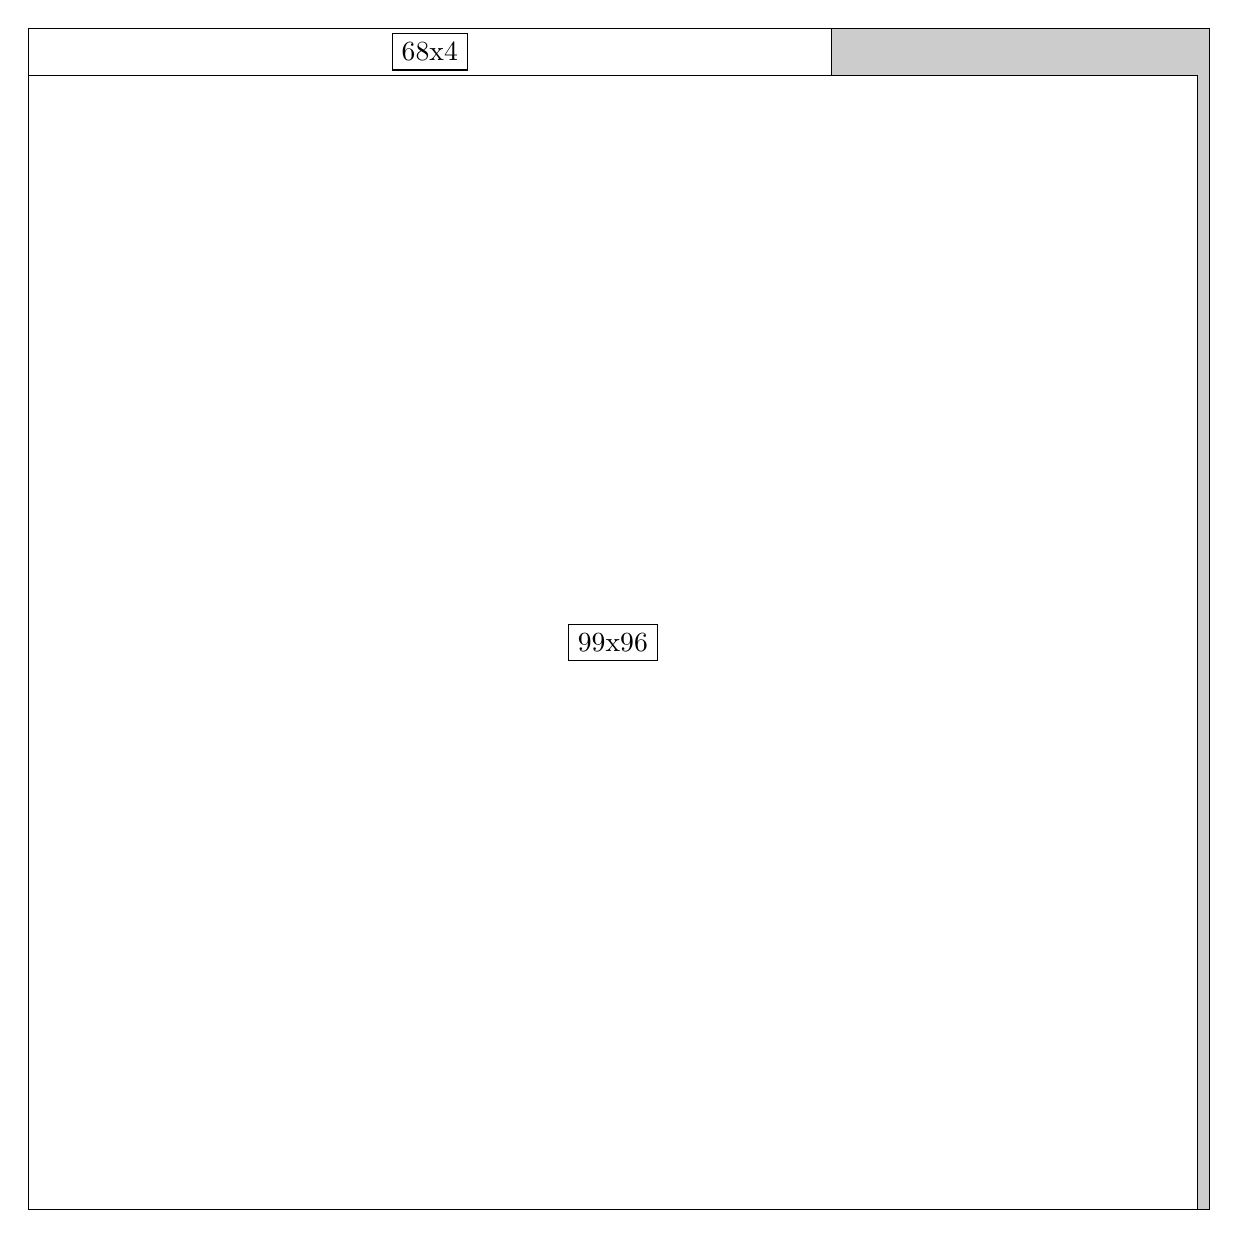
\begin{tikzpicture}[shorten >=1pt,scale=1.0,every node/.style={scale=1.0},->]
\tikzstyle{vertex}=[circle,fill=black!25,minimum size=14pt,inner sep=0pt]
\filldraw[fill=gray!40!white, draw=black] (0,0) rectangle (15.0,15.0);
\foreach \name/\x/\y/\w/\h in {99x96/0.0/0.0/14.85/14.399999999999999,68x4/0.0/14.399999999999999/10.2/0.6}
\filldraw[fill=white!40!white, draw=black] (\x,\y) rectangle node[draw] (\name) {\name} ++(\w,\h);
\end{tikzpicture}


w =99 , h =96 , x =0 , y =0 , v =9504
\par
w =68 , h =4 , x =0 , y =96 , v =272
\par
\newpage


\begin{tikzpicture}[shorten >=1pt,scale=1.0,every node/.style={scale=1.0},->]
\tikzstyle{vertex}=[circle,fill=black!25,minimum size=14pt,inner sep=0pt]
\filldraw[fill=gray!40!white, draw=black] (0,0) rectangle (15.0,15.0);
\foreach \name/\x/\y/\w/\h in {100x93/0.0/0.0/15.0/13.95,95x7/0.0/13.95/14.25/1.05}
\filldraw[fill=white!40!white, draw=black] (\x,\y) rectangle node[draw] (\name) {\name} ++(\w,\h);
\end{tikzpicture}


w =100 , h =93 , x =0 , y =0 , v =9300
\par
w =95 , h =7 , x =0 , y =93 , v =665
\par
\newpage


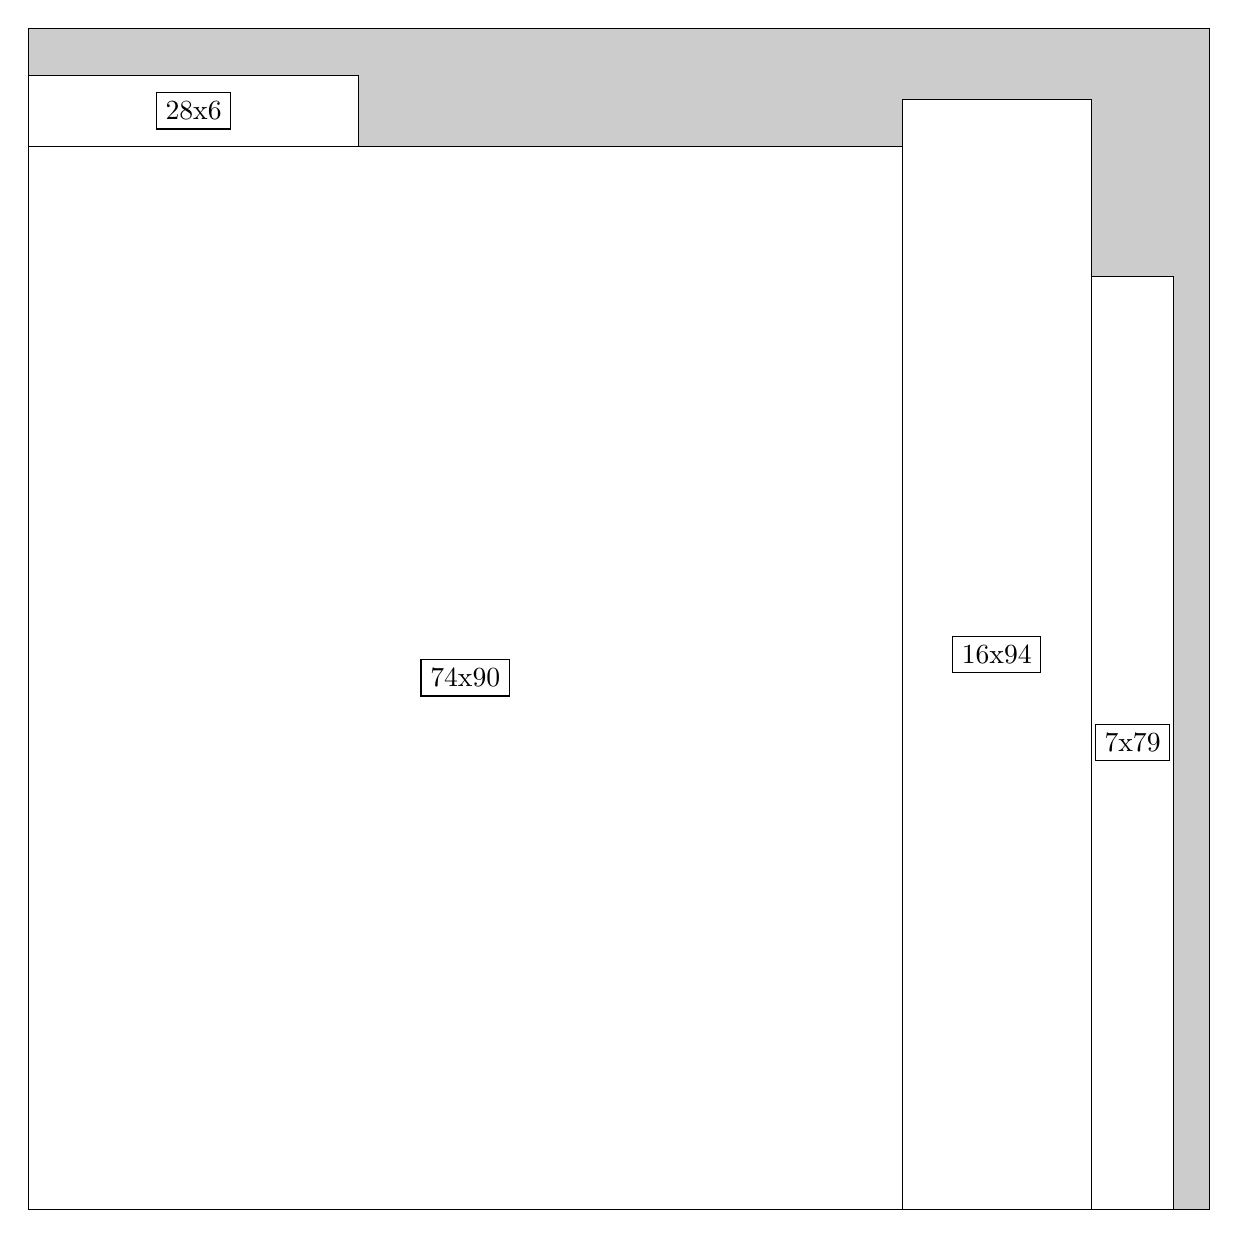
\begin{tikzpicture}[shorten >=1pt,scale=1.0,every node/.style={scale=1.0},->]
\tikzstyle{vertex}=[circle,fill=black!25,minimum size=14pt,inner sep=0pt]
\filldraw[fill=gray!40!white, draw=black] (0,0) rectangle (15.0,15.0);
\foreach \name/\x/\y/\w/\h in {74x90/0.0/0.0/11.1/13.5,16x94/11.1/0.0/2.4/14.1,7x79/13.5/0.0/1.05/11.85,28x6/0.0/13.5/4.2/0.8999999999999999}
\filldraw[fill=white!40!white, draw=black] (\x,\y) rectangle node[draw] (\name) {\name} ++(\w,\h);
\end{tikzpicture}


w =74 , h =90 , x =0 , y =0 , v =6660
\par
w =16 , h =94 , x =74 , y =0 , v =1504
\par
w =7 , h =79 , x =90 , y =0 , v =553
\par
w =28 , h =6 , x =0 , y =90 , v =168
\par
\newpage


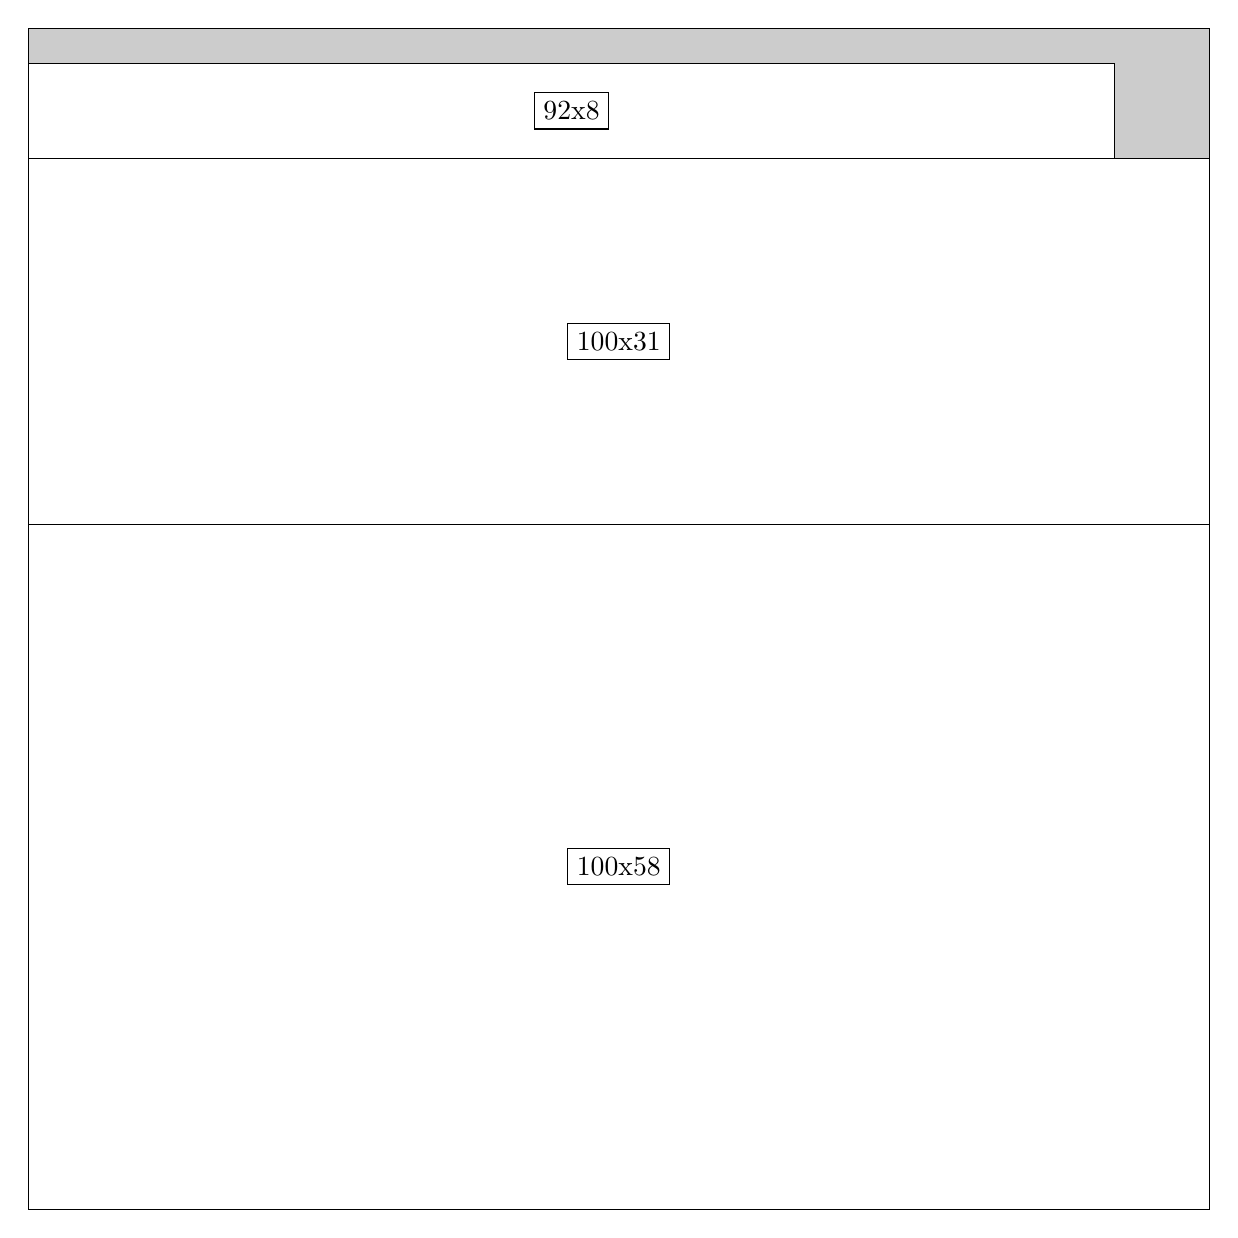
\begin{tikzpicture}[shorten >=1pt,scale=1.0,every node/.style={scale=1.0},->]
\tikzstyle{vertex}=[circle,fill=black!25,minimum size=14pt,inner sep=0pt]
\filldraw[fill=gray!40!white, draw=black] (0,0) rectangle (15.0,15.0);
\foreach \name/\x/\y/\w/\h in {100x58/0.0/0.0/15.0/8.7,100x31/0.0/8.7/15.0/4.6499999999999995,92x8/0.0/13.35/13.799999999999999/1.2}
\filldraw[fill=white!40!white, draw=black] (\x,\y) rectangle node[draw] (\name) {\name} ++(\w,\h);
\end{tikzpicture}


w =100 , h =58 , x =0 , y =0 , v =5800
\par
w =100 , h =31 , x =0 , y =58 , v =3100
\par
w =92 , h =8 , x =0 , y =89 , v =736
\par
\newpage


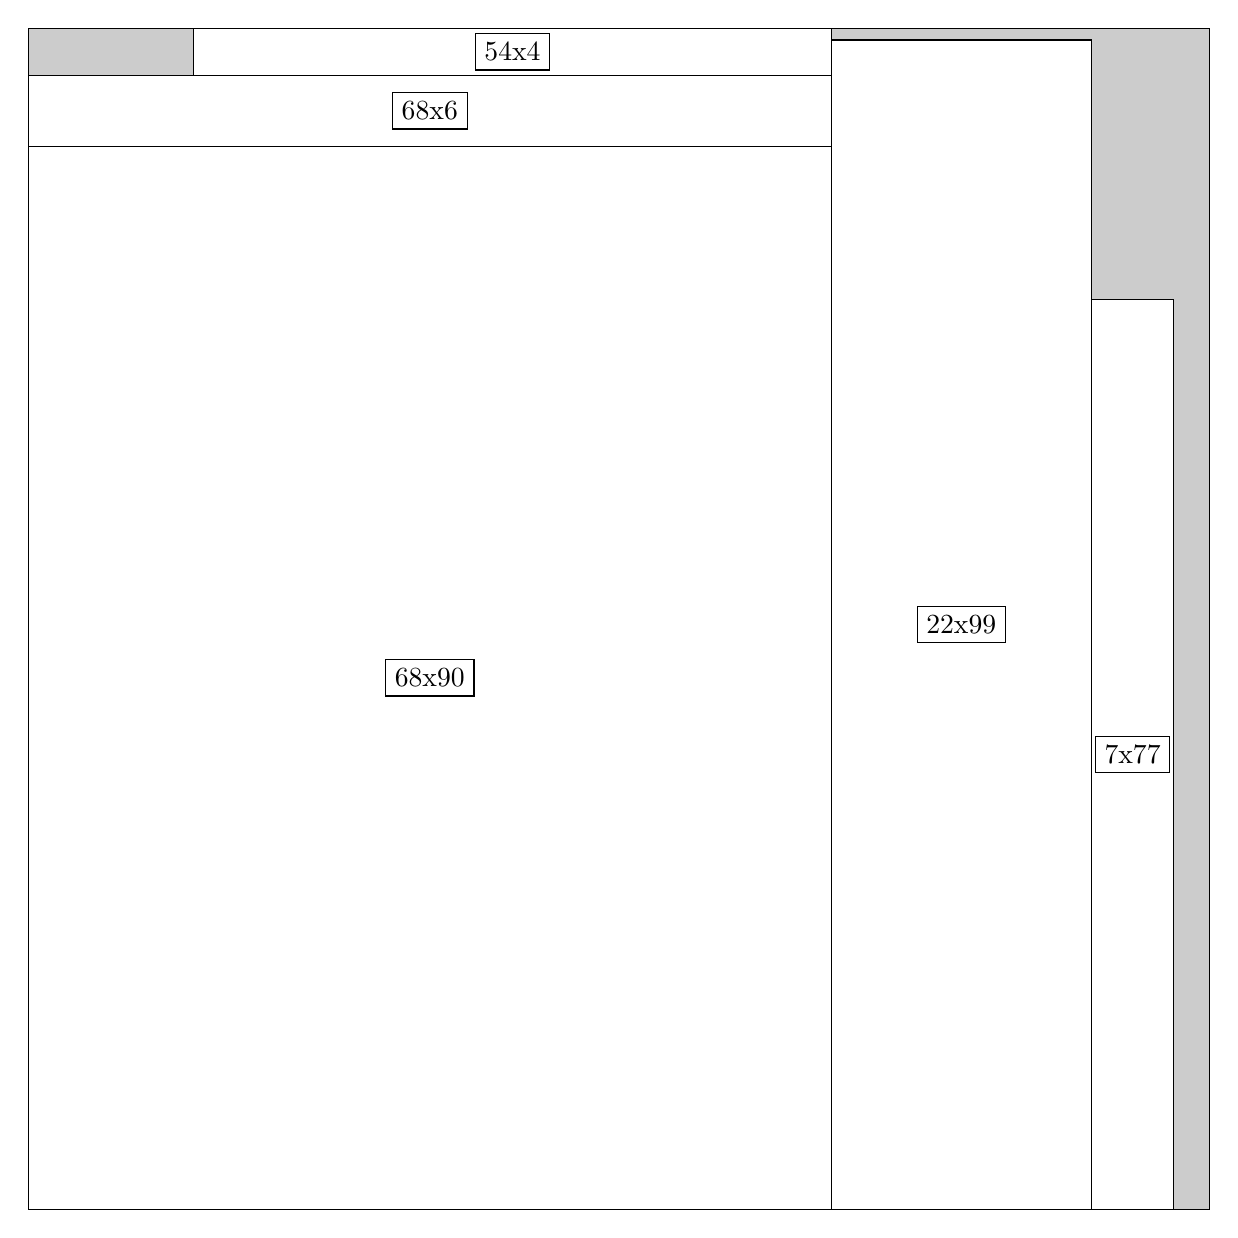
\begin{tikzpicture}[shorten >=1pt,scale=1.0,every node/.style={scale=1.0},->]
\tikzstyle{vertex}=[circle,fill=black!25,minimum size=14pt,inner sep=0pt]
\filldraw[fill=gray!40!white, draw=black] (0,0) rectangle (15.0,15.0);
\foreach \name/\x/\y/\w/\h in {68x90/0.0/0.0/10.2/13.5,22x99/10.2/0.0/3.3/14.85,7x77/13.5/0.0/1.05/11.549999999999999,68x6/0.0/13.5/10.2/0.8999999999999999,54x4/2.1/14.399999999999999/8.1/0.6}
\filldraw[fill=white!40!white, draw=black] (\x,\y) rectangle node[draw] (\name) {\name} ++(\w,\h);
\end{tikzpicture}


w =68 , h =90 , x =0 , y =0 , v =6120
\par
w =22 , h =99 , x =68 , y =0 , v =2178
\par
w =7 , h =77 , x =90 , y =0 , v =539
\par
w =68 , h =6 , x =0 , y =90 , v =408
\par
w =54 , h =4 , x =14 , y =96 , v =216
\par
\newpage


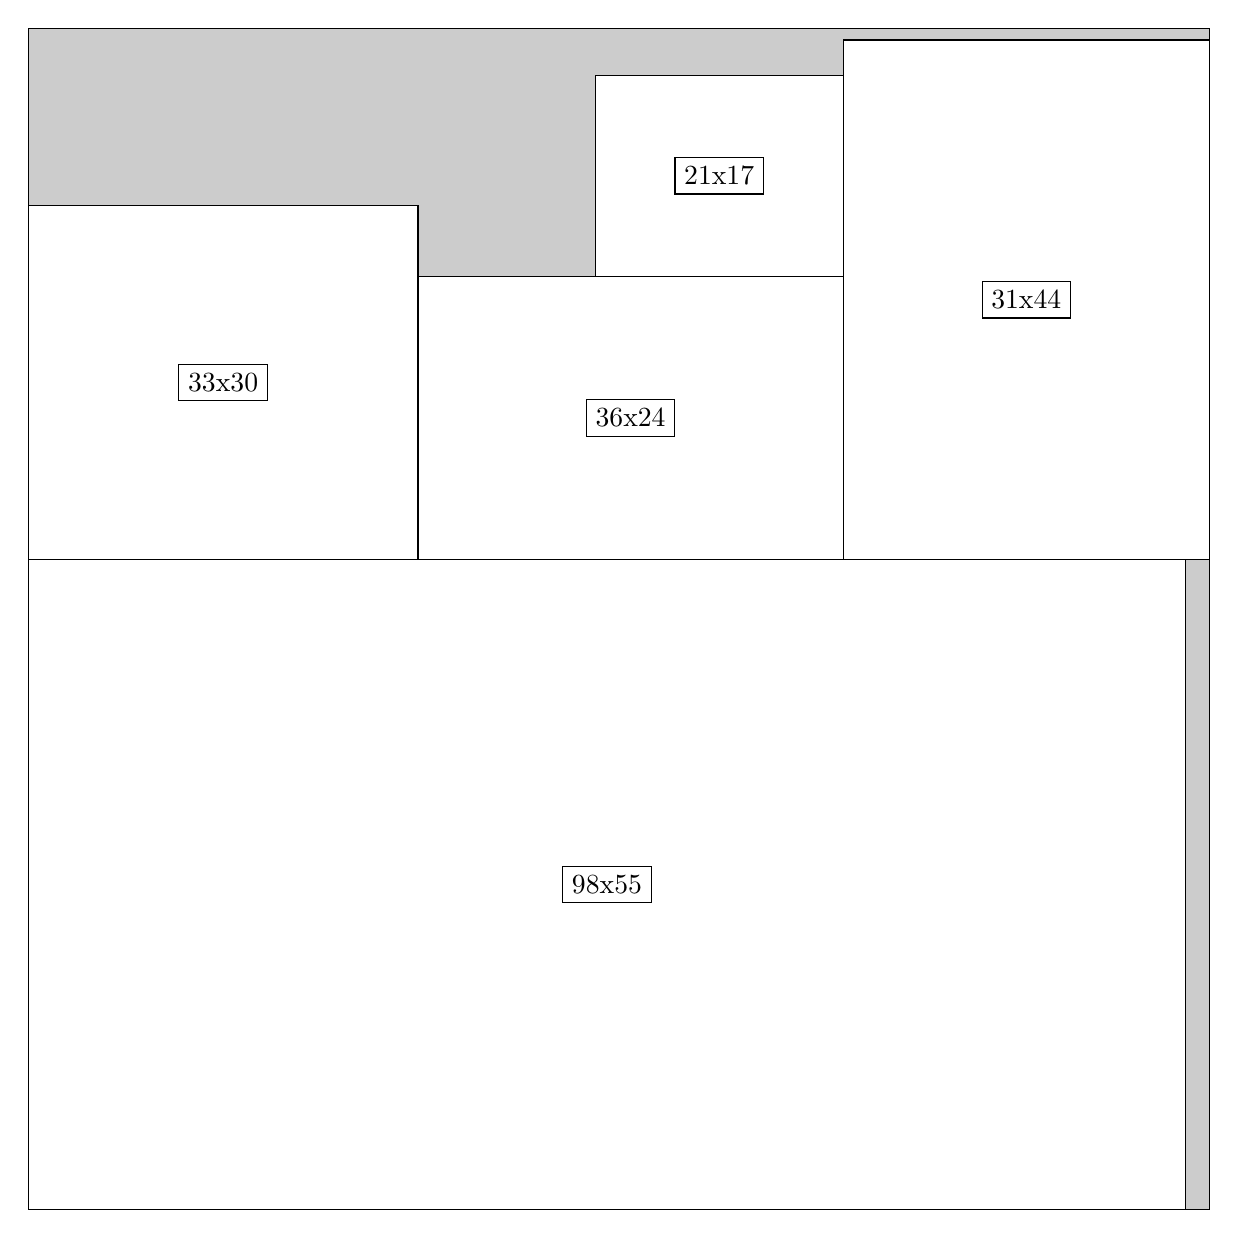
\begin{tikzpicture}[shorten >=1pt,scale=1.0,every node/.style={scale=1.0},->]
\tikzstyle{vertex}=[circle,fill=black!25,minimum size=14pt,inner sep=0pt]
\filldraw[fill=gray!40!white, draw=black] (0,0) rectangle (15.0,15.0);
\foreach \name/\x/\y/\w/\h in {98x55/0.0/0.0/14.7/8.25,33x30/0.0/8.25/4.95/4.5,31x44/10.35/8.25/4.6499999999999995/6.6,36x24/4.95/8.25/5.3999999999999995/3.5999999999999996,21x17/7.199999999999999/11.85/3.15/2.55}
\filldraw[fill=white!40!white, draw=black] (\x,\y) rectangle node[draw] (\name) {\name} ++(\w,\h);
\end{tikzpicture}


w =98 , h =55 , x =0 , y =0 , v =5390
\par
w =33 , h =30 , x =0 , y =55 , v =990
\par
w =31 , h =44 , x =69 , y =55 , v =1364
\par
w =36 , h =24 , x =33 , y =55 , v =864
\par
w =21 , h =17 , x =48 , y =79 , v =357
\par
\newpage


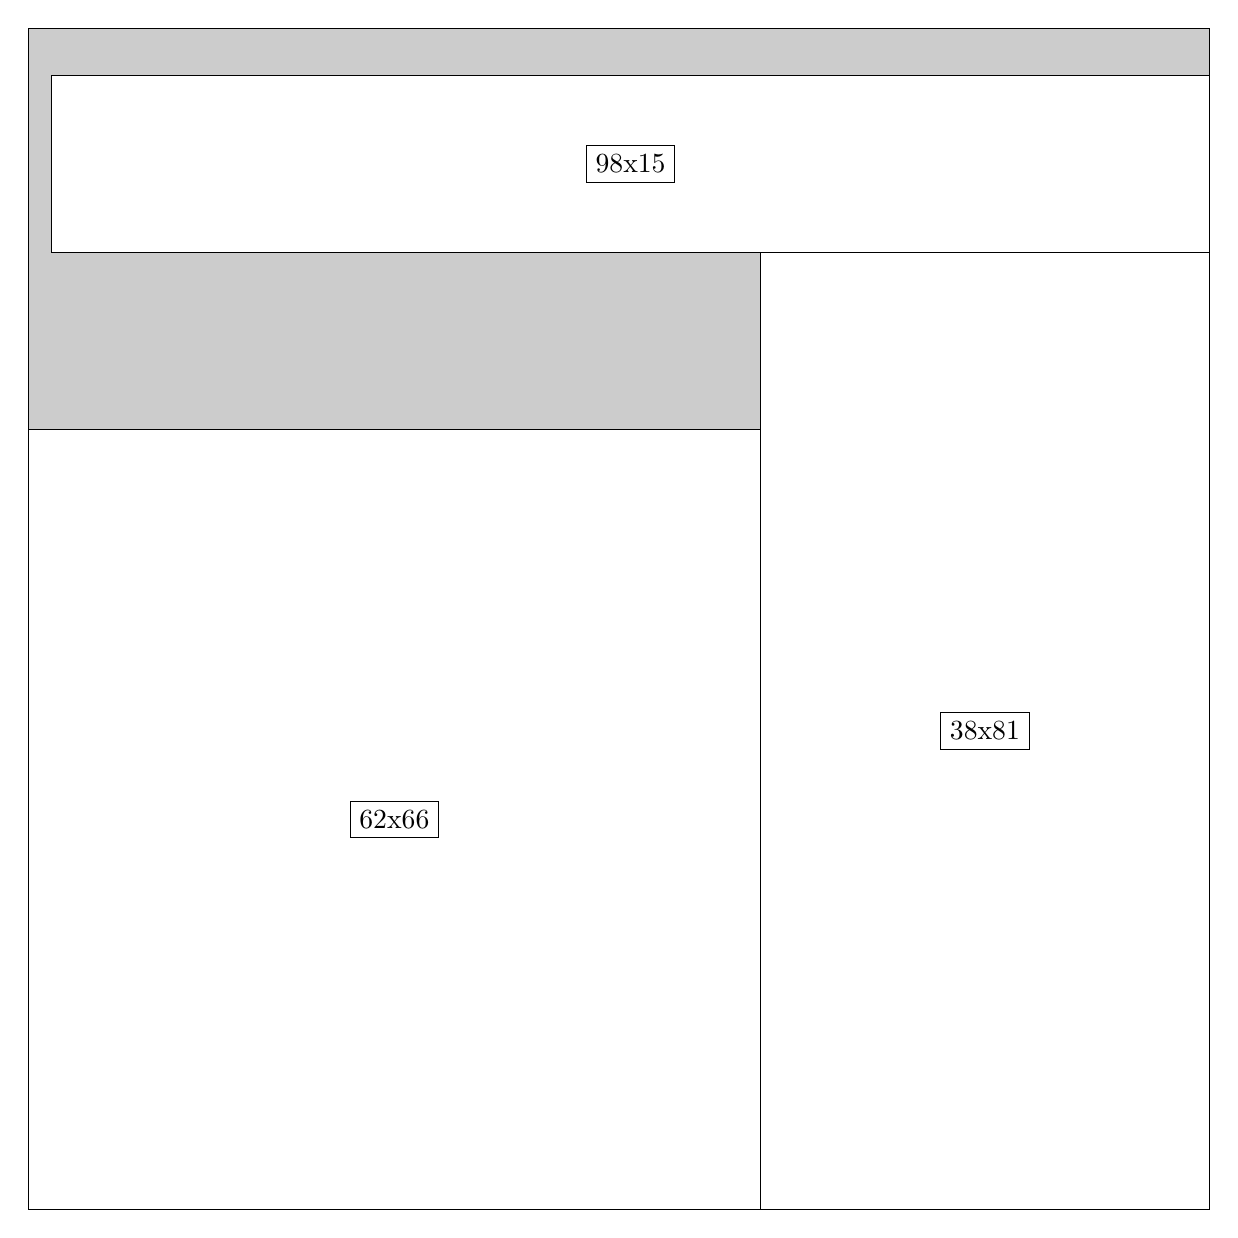
\begin{tikzpicture}[shorten >=1pt,scale=1.0,every node/.style={scale=1.0},->]
\tikzstyle{vertex}=[circle,fill=black!25,minimum size=14pt,inner sep=0pt]
\filldraw[fill=gray!40!white, draw=black] (0,0) rectangle (15.0,15.0);
\foreach \name/\x/\y/\w/\h in {62x66/0.0/0.0/9.299999999999999/9.9,38x81/9.299999999999999/0.0/5.7/12.15,98x15/0.3/12.15/14.7/2.25}
\filldraw[fill=white!40!white, draw=black] (\x,\y) rectangle node[draw] (\name) {\name} ++(\w,\h);
\end{tikzpicture}


w =62 , h =66 , x =0 , y =0 , v =4092
\par
w =38 , h =81 , x =62 , y =0 , v =3078
\par
w =98 , h =15 , x =2 , y =81 , v =1470
\par
\newpage


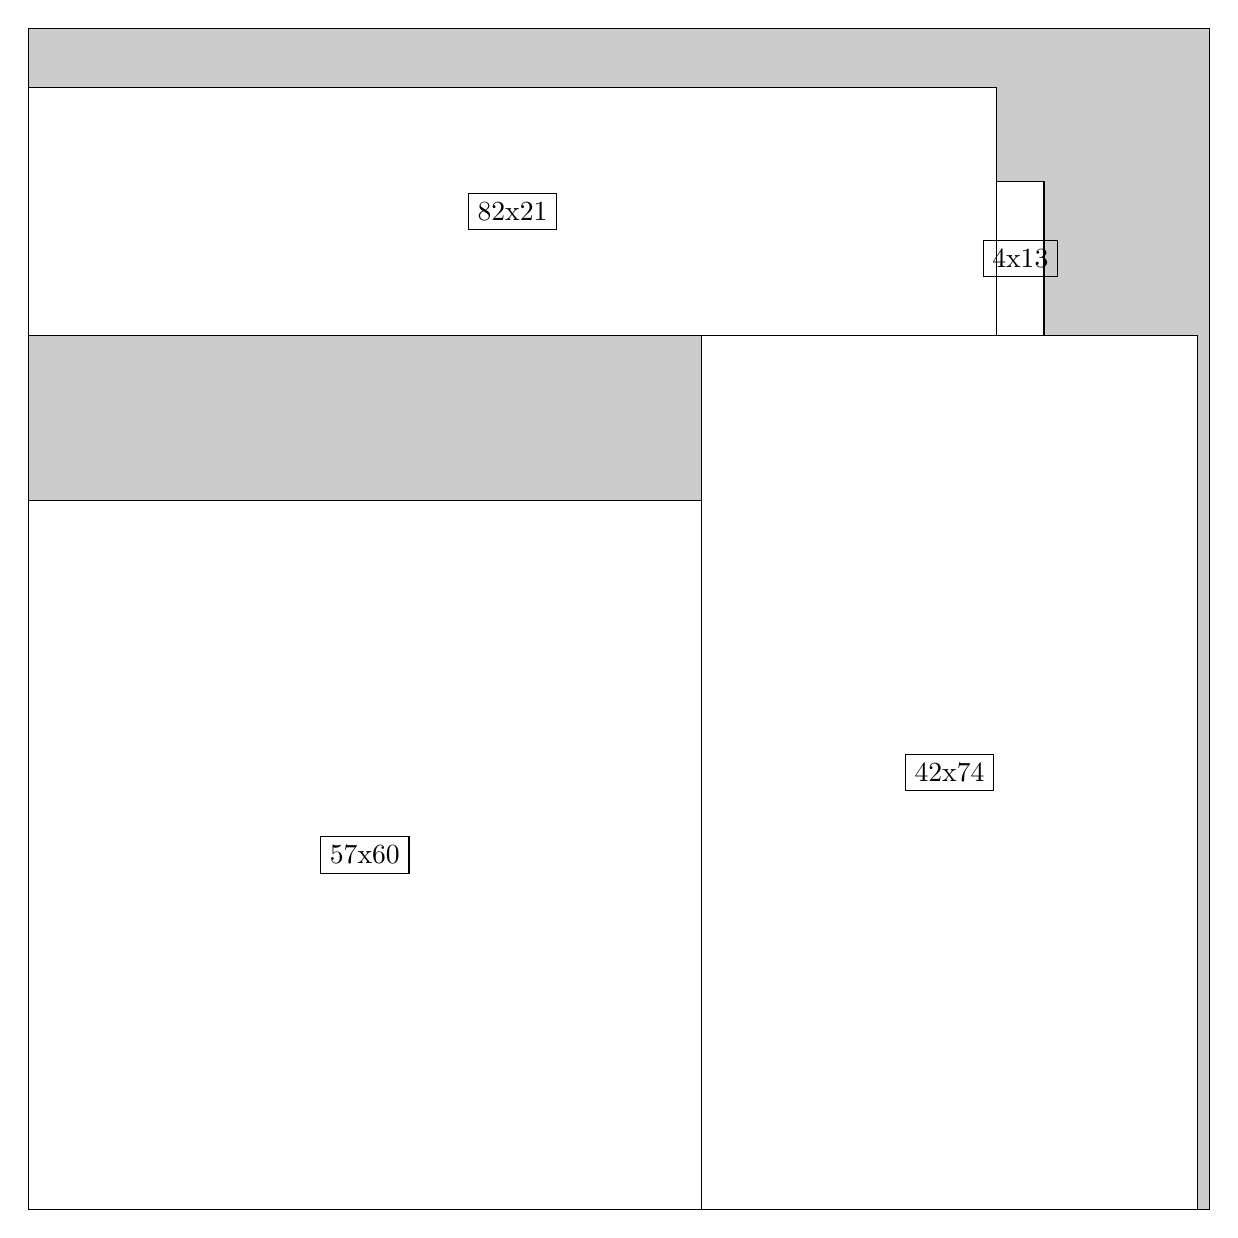
\begin{tikzpicture}[shorten >=1pt,scale=1.0,every node/.style={scale=1.0},->]
\tikzstyle{vertex}=[circle,fill=black!25,minimum size=14pt,inner sep=0pt]
\filldraw[fill=gray!40!white, draw=black] (0,0) rectangle (15.0,15.0);
\foreach \name/\x/\y/\w/\h in {57x60/0.0/0.0/8.549999999999999/9.0,42x74/8.549999999999999/0.0/6.3/11.1,82x21/0.0/11.1/12.299999999999999/3.15,4x13/12.299999999999999/11.1/0.6/1.95}
\filldraw[fill=white!40!white, draw=black] (\x,\y) rectangle node[draw] (\name) {\name} ++(\w,\h);
\end{tikzpicture}


w =57 , h =60 , x =0 , y =0 , v =3420
\par
w =42 , h =74 , x =57 , y =0 , v =3108
\par
w =82 , h =21 , x =0 , y =74 , v =1722
\par
w =4 , h =13 , x =82 , y =74 , v =52
\par
\newpage


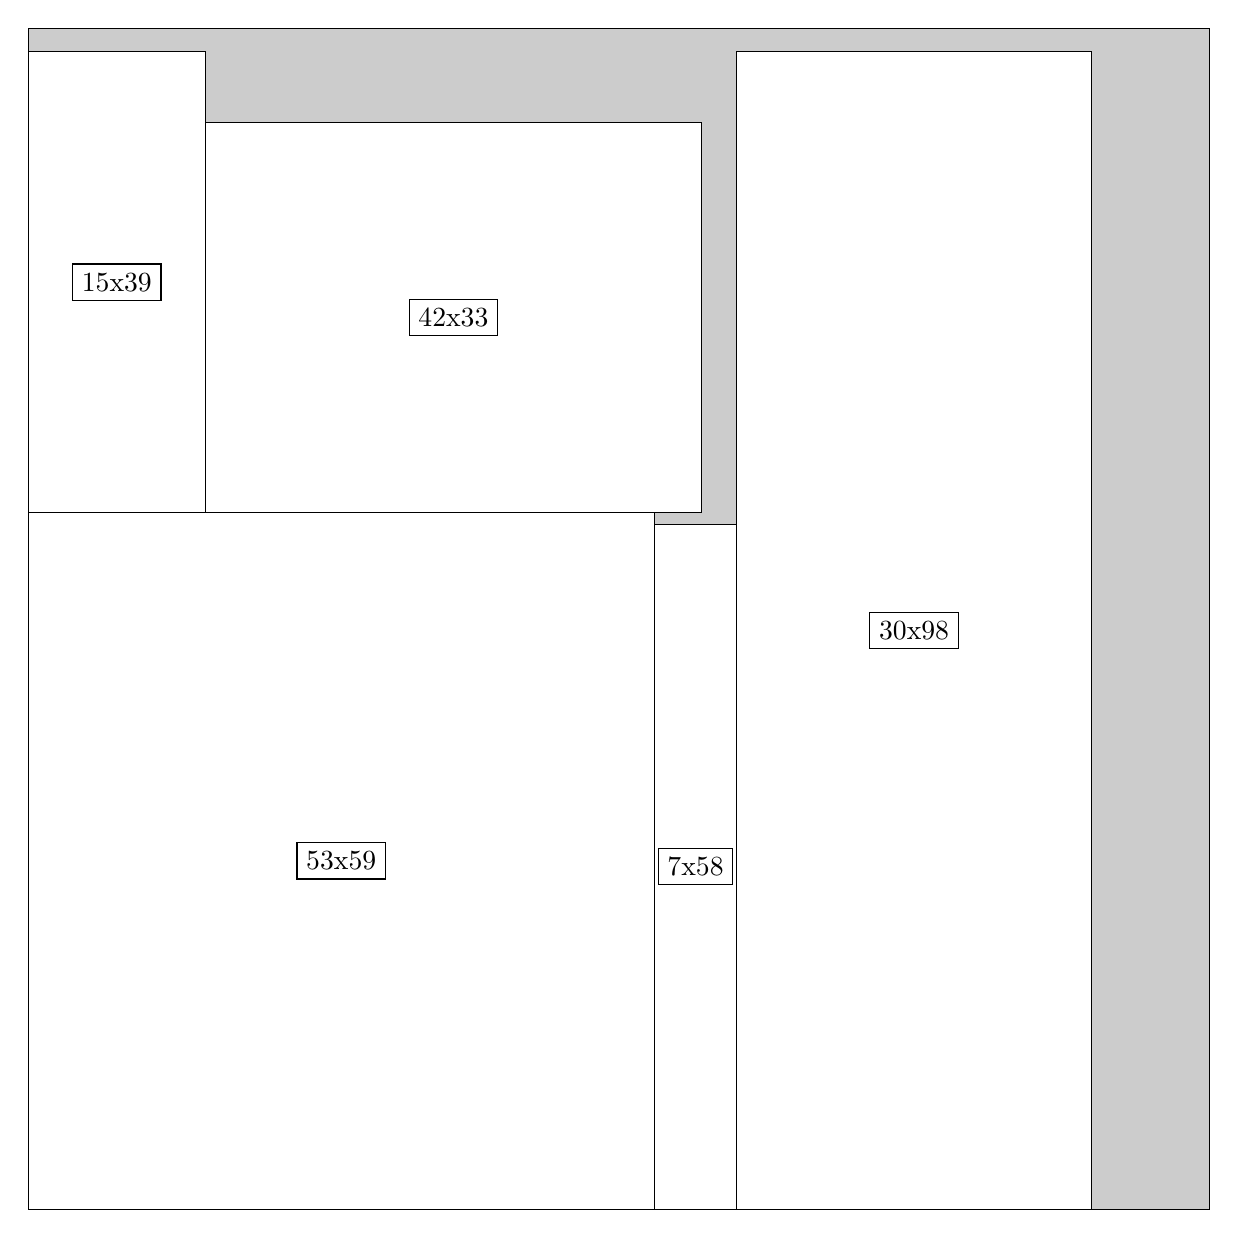
\begin{tikzpicture}[shorten >=1pt,scale=1.0,every node/.style={scale=1.0},->]
\tikzstyle{vertex}=[circle,fill=black!25,minimum size=14pt,inner sep=0pt]
\filldraw[fill=gray!40!white, draw=black] (0,0) rectangle (15.0,15.0);
\foreach \name/\x/\y/\w/\h in {53x59/0.0/0.0/7.949999999999999/8.85,30x98/9.0/0.0/4.5/14.7,42x33/2.25/8.85/6.3/4.95,15x39/0.0/8.85/2.25/5.85,7x58/7.949999999999999/0.0/1.05/8.7}
\filldraw[fill=white!40!white, draw=black] (\x,\y) rectangle node[draw] (\name) {\name} ++(\w,\h);
\end{tikzpicture}


w =53 , h =59 , x =0 , y =0 , v =3127
\par
w =30 , h =98 , x =60 , y =0 , v =2940
\par
w =42 , h =33 , x =15 , y =59 , v =1386
\par
w =15 , h =39 , x =0 , y =59 , v =585
\par
w =7 , h =58 , x =53 , y =0 , v =406
\par
\newpage


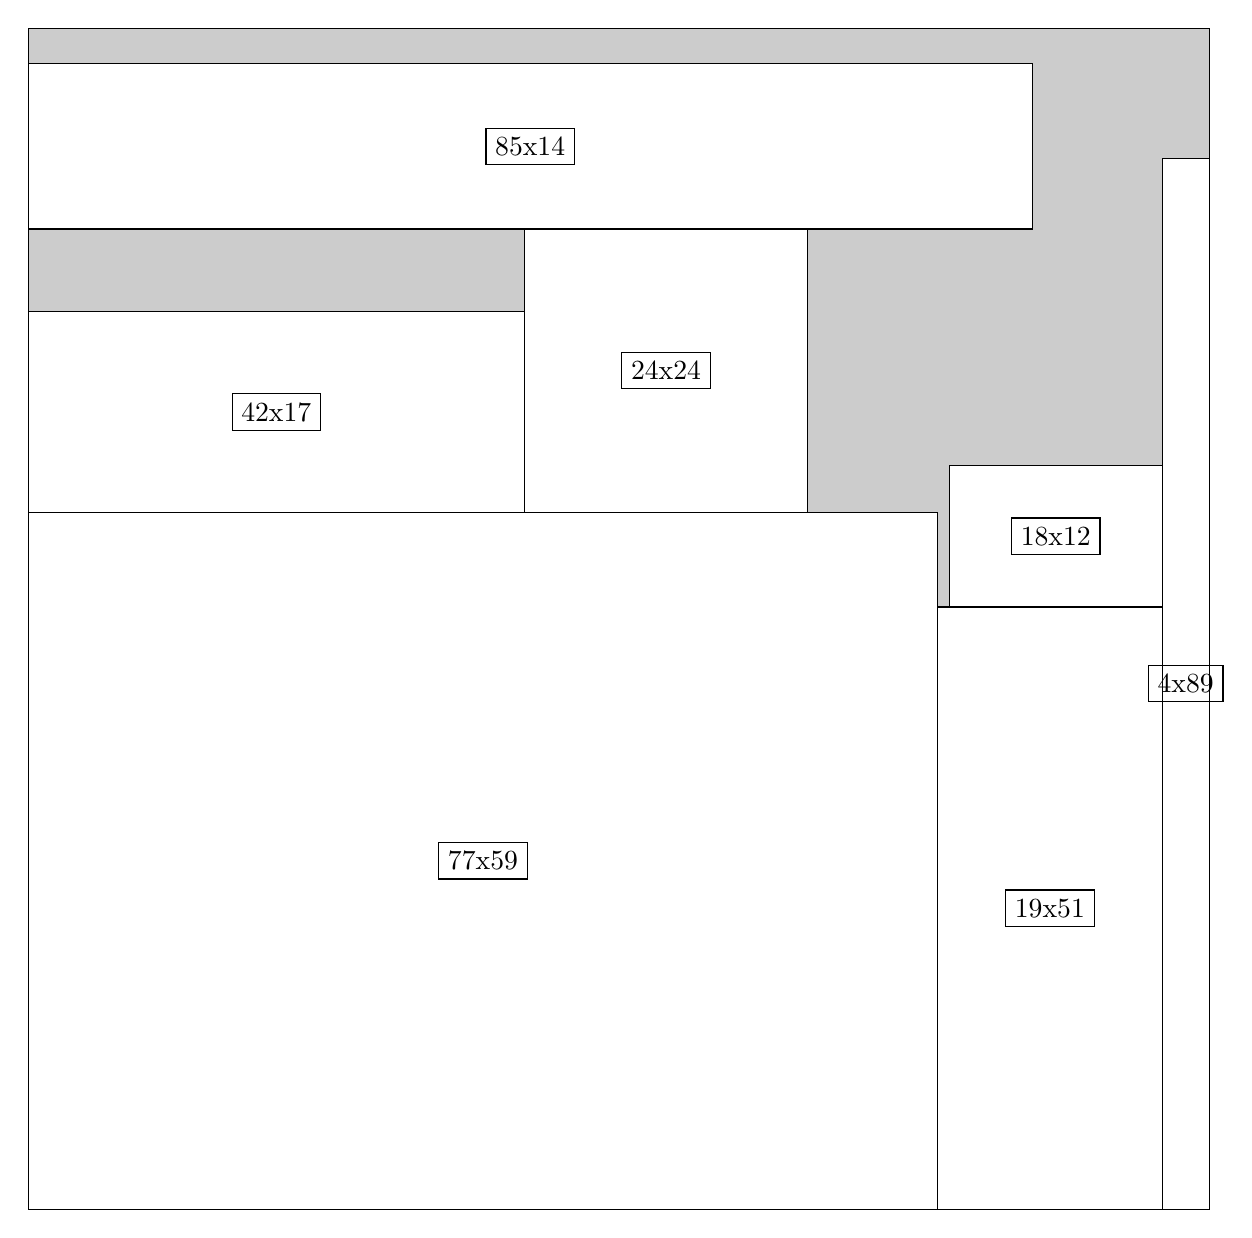
\begin{tikzpicture}[shorten >=1pt,scale=1.0,every node/.style={scale=1.0},->]
\tikzstyle{vertex}=[circle,fill=black!25,minimum size=14pt,inner sep=0pt]
\filldraw[fill=gray!40!white, draw=black] (0,0) rectangle (15.0,15.0);
\foreach \name/\x/\y/\w/\h in {85x14/0.0/12.45/12.75/2.1,77x59/0.0/0.0/11.549999999999999/8.85,19x51/11.549999999999999/0.0/2.85/7.6499999999999995,42x17/0.0/8.85/6.3/2.55,24x24/6.3/8.85/3.5999999999999996/3.5999999999999996,4x89/14.399999999999999/0.0/0.6/13.35,18x12/11.7/7.6499999999999995/2.6999999999999997/1.7999999999999998}
\filldraw[fill=white!40!white, draw=black] (\x,\y) rectangle node[draw] (\name) {\name} ++(\w,\h);
\end{tikzpicture}


w =85 , h =14 , x =0 , y =83 , v =1190
\par
w =77 , h =59 , x =0 , y =0 , v =4543
\par
w =19 , h =51 , x =77 , y =0 , v =969
\par
w =42 , h =17 , x =0 , y =59 , v =714
\par
w =24 , h =24 , x =42 , y =59 , v =576
\par
w =4 , h =89 , x =96 , y =0 , v =356
\par
w =18 , h =12 , x =78 , y =51 , v =216
\par
\newpage


\end{document}